Encuentra el volumen acotado por la gráfica de 
$f(x,y)=1+2x+3y$, el rectángulo 
$[1,2]\times [0,1]$, y los cuatro lados verticales del rectángulo 
$R$
como en la figura
\begin{figure}[H]
    \begin{center}
        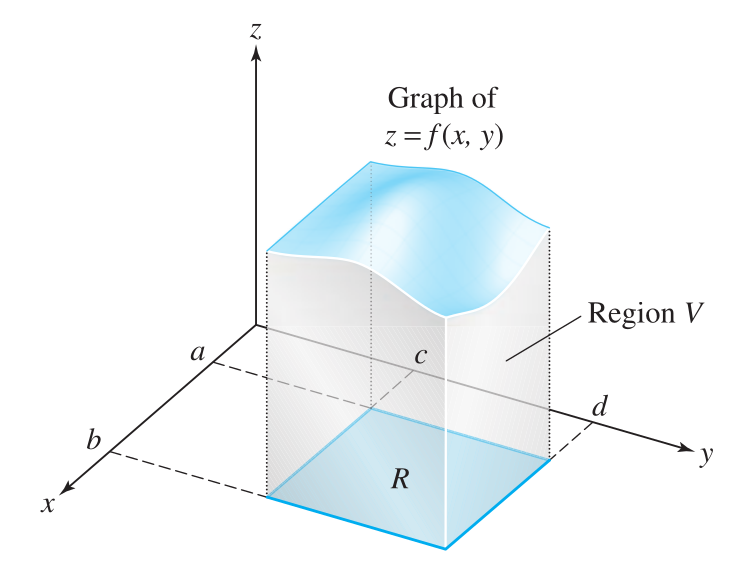
\includegraphics[width=0.3\textwidth]{img/Ej2/ej14.png}
    \end{center}
\end{figure}
\begin{solution}
%     La gráfica de esta función es un plano por lo que su máximo está ubicado en la frontera
%     del dominio de $f$. Pero por la fórmula de $f$ es fácil ver que mientras más grande sea 
%     $x$ y más grande sea $y$ se alcanzará el máximo en el punto
%     en el punto $(2,1)$, dejando como tal máximo a \( f(2,1)=8 \).
%     Igualmente podemos deducir que el mínimo de \( f \) está en \( (1,0) \) con su valor de 
%     \( f(1,0)=3>0 \). 
% 
    Podemos ver las intersecciones de los planos paralelos al plano \( yz \) y dependiendo 
    del valor de $x$, podemos ver que estos tienen
    área
    \[ \int_{0}^1 1+2x+3y \, dy = \left. \left[ y+2xy+3 \frac{y^2}{2} \right] \right\rvert_0^1 =
    \frac{5}{2} +2x.\] 
    Luego, por Cavalieri,  el volumen de la figura entera es 
    \begin{align*}
        \int_1^2
        \frac{5}{2} +2x \, dx
        &=
        \left.
        \left[ \frac{5}{2} x + x^2 \right] \right\rvert_1^2\\
        &=
        5+4- \frac{5}{2} - 1\\
        &=
        \frac{11}{2}.
    \end{align*}
\end{solution}
